\section{Framework Design}
\textbf{Architecture.} The framework applies policies to the packets that carry
an operation. Ingress identifies the request, its TCP acknowledgment and its
application response. The traffic manager holds packets behind internal blocker
reservoirs. Returning packets pass through ingress again before they are released
or queued. Egress forwards a released packet or produces the supported response
segments. Blockers remain inside the switch; a cloned request triggers their
generation and is not itself a reservoir.

\begin{figure*}[t]
\centering
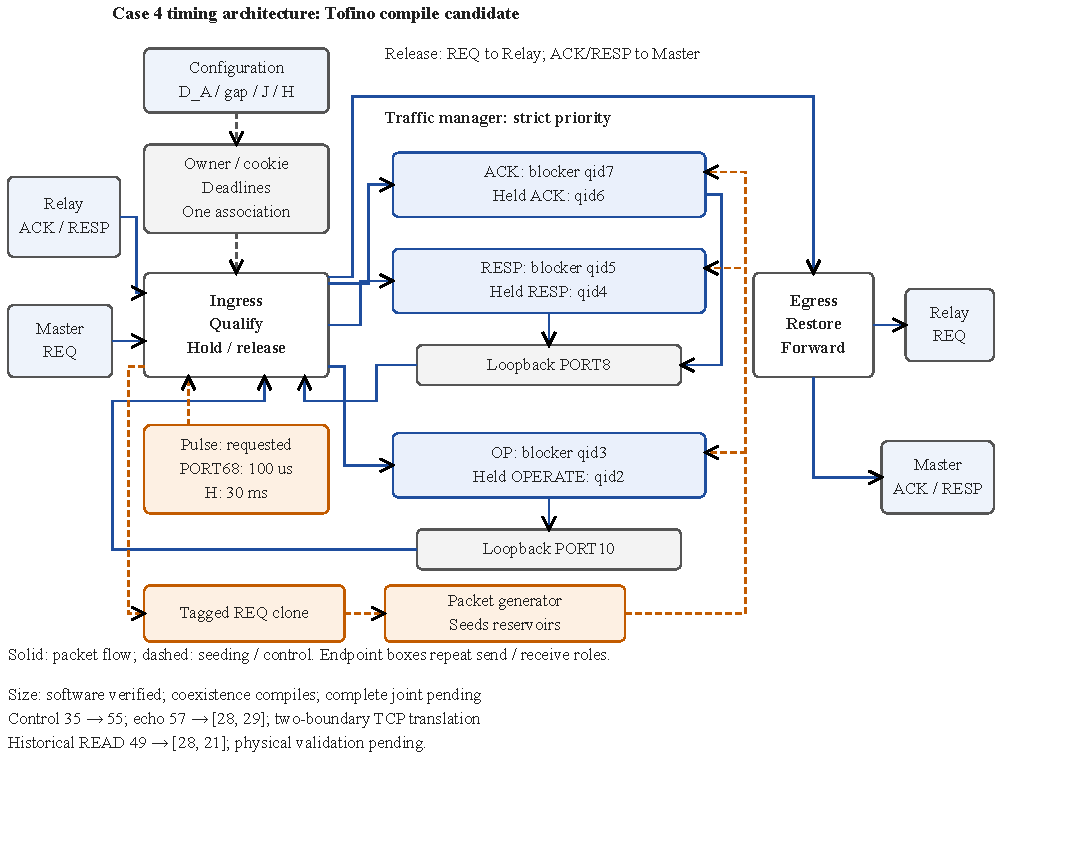
\includegraphics[width=\textwidth]{../figures/fig_framework_mechanism.pdf}
\caption{Working mechanism and separate size component. The read and control
scheduling domains return through ingress. The size branch is not evidence of a
complete joint Tofino implementation. Source, queue mapping and rendering
provenance accompany the editable figure.}
\label{fig:mechanism}
\end{figure*}

\textbf{Operation-related policies.} A response has a generic DNP3 RESPONSE
function, so the owner request determines its parent operation. READ, SELECT and
OPERATE remain separate populations. SELECT and OPERATE form two phases of
select-before-operate (SBO); a response segment inherits its parent's operation.
For an eligible control request, the size policy appends a configured inert
command object while retaining every real object and its fields. It repeats the
same transformation on the matching OPERATE. Response splitting changes TCP
segmentation, not the application message. The policy requires successful real
and decoy statuses and a verified inert-point configuration.

\textbf{Case 4 composition.} An early response waits until its acknowledgment
can leave. A late response becomes the readiness event for acknowledgment release.
After normal acknowledgment commitment, the response waits the full configured
gap. In an ideal schedule, with request arrival $t_0$, native acknowledgment
arrival $t_A$, complete associated response availability $t_R$, request-relative
acknowledgment deadline $D_A$, and physical departures $e_A,e_R$,
\begin{align}
e_A&=\max(t_0+D_A,t_A,t_R),\\
e_R&=e_A+\mathrm{configured\ CLRT}_{new}.
\end{align}
The acknowledgment hold is $e_A-t_A$, and the response hold is $e_R-t_R$.
Consequently, subtracting only the native acknowledgment-to-response interval
from $D_A$ omits the request-to-acknowledgment interval. The implementation starts
the response deadline at qualified loopback commitment, an internal reference
that remains distinct from measured physical departure.

\textbf{Finite recovery.} A 30 ms readiness expiry advances independently of
both reservoirs. If readiness fails, the switch releases held originals without
fabricating an acknowledgment or response. A normal ACK commitment invalidates
an in-flight readiness scan and preserves the future response deadline. Packet
ordering near expiry can still select explicit fallback before commitment.
Completion, stale-packet rejection and next-owner admission need separate checks;
an event-model timer does not establish physical queue drain.

\textbf{Parameter constraints.} Admission accounts for the complete feedback
interval each sender's timer spans, application and SBO deadlines, detection,
drain and release. TCP's retransmission timer is not remaining headroom at switch
arrival~\cite{case4_rfc6298}. Missing measurements keep admission provisional.
The policy study retains $D_A\in\{5,10,15,20\}$ ms and configured
$\mathrm{CLRT}_{new}=1$ ms, subject to a fixed 40 ms cap. The declared hardware
accuracy criteria are not software timing tolerances or achieved results.

\textbf{Other policy capabilities.} ACK-focused scheduling moves
request-to-ACK timing toward response readiness. Response-focused scheduling
holds only responses that arrive inside its window. A generated-ACK prototype
accepts responsibility for downstream loss and remains incomplete. These three
cases are explanation-only history in this assignment; Case 4 is the new target.
